\section{The model}
\label{sec:the-model}
In this section we will go through the model presented in \cite{self-org} in 
detail. As mentioned in the introduction, social force models are agent-based, 
that is they describe the system by looking at the behaviour of each agent or, 
in our case, pedestrian in the system.


In this model the behaviour each pedestrian is defined by a series of social 
forces. We will describe three main forces, that each represent a tendency of 
the pedestrians. These forces are \emph{the desired movement force},  
\emph{the interaction force} between pedestrians and \emph{the repulsive 
force}  from the walls. The model also contains an attractive force, allowing 
e.g. a group of pedestrians to stick together when moving around, and a 
fluctuation term, adding a stochastic quality to the model. Both these forces, 
however, are only mentioned in the article, and are not really used. We have 
written the authors of the article asking about this, and they have replied 
that these parts of the model have not been used in practice, but that they 
might be useful to include at a later point in time.  Because of this, we will 
exclude these parts from the explanation of the model.

In the following, we will go through the three main forces, explaining how 
they are calculated. Since the notation used in the article is ambiguous and 
confusing, we introduce our own notation in an attempt to make it clearer. We 
will not refer to the original notation, but only use our own.

In the model, a pedestrian is represented by a circle with a centre, a radius 
and a current velocity. Walls are represented as line segments. The desired 
direction is represented by assigning to each pedestrian a target to move 
towards. Various other parameters are assigned to each pedestrian; these will 
be explained when relevant throughout the description. The notation for 
pedestrians and the main forces acting on a pedestrian are illustrated in  
figure~\ref{pedestrian-notation}.  

\begin{figure}[ht]
    \centering
    \subfloat[Notation of pedestrian properties.]{
        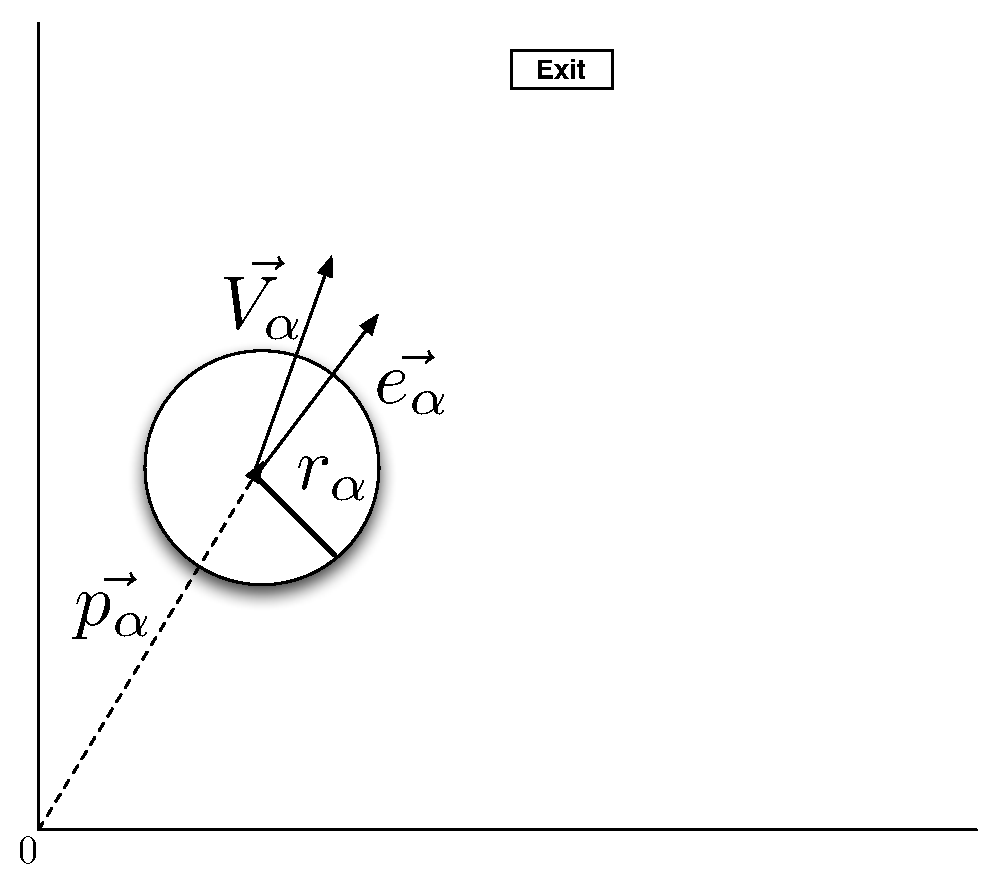
\includegraphics[width=0.45\textwidth]{Figures/NotationOfPedestrian.pdf}
        \label{subfig:notation}
    }
    \subfloat[Main forces acting on a pedestrian.]{
        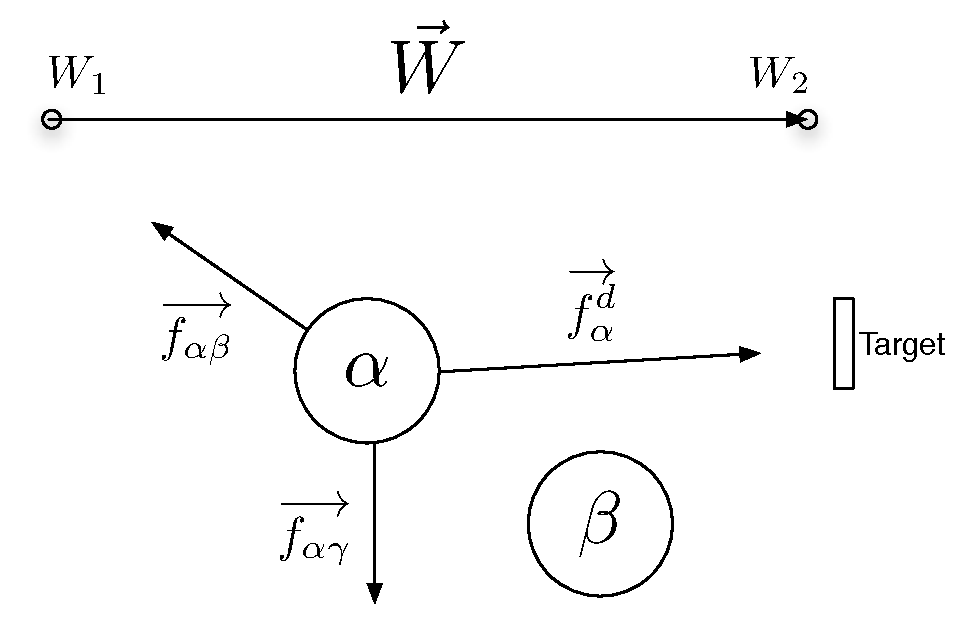
\includegraphics[width=0.45\textwidth]{Figures/ForceModel.pdf}
        \label{subfig:forces}
    }
    \caption[Notation for pedestrians]{Notation for a pedestrian.  
    \subref{subfig:notation} The notation for pedestrian properties. Position 
    vector ($ \overrightarrow{p_{\alpha}} $), velocity vector ($ 
    \overrightarrow{V_{\alpha}} $), vector pointing towards 
    the target ($\overrightarrow{e_{\alpha}}$)  and radius ($ R_{\alpha} $).
    %
    \subref{subfig:forces} Main forces acting on a pedestrian $\alpha$. 
    Repulsive force from pedestrian $\beta$ 
    ($\overrightarrow{f_{\alpha\beta}}$), repulsive force from wall $\gamma$ 
    ($\overrightarrow{f_{\alpha \gamma}}$) and desired force towards target 
    ($\overrightarrow{f^{d}_{\alpha}}$).}

    \label{pedestrian-notation}
\end{figure}

The resulting force for pedestrian $\alpha$, $\overrightarrow{f_{\alpha}}$ is 
the sum of the three main forces.

\begin{equation}\label{model}
    \overrightarrow{f_{\alpha}} = \overrightarrow{f^{d}_{\alpha}} +
    \sum_{\gamma} \overrightarrow{f_{\alpha \gamma}} +
    \sum_{\beta \neq \alpha} \overrightarrow{f_{\alpha \beta}}
\end{equation}

Here $\overrightarrow{f_{\alpha}^{d}}$ is the desired force, 
$\overrightarrow{f_{\alpha \gamma}}$ is the repulsive force from wall $\gamma$ 
and $\overrightarrow{f_{\alpha \beta}}$ is the repulsive force from pedestrian 
$\beta$. The main forces are summarised in table~\ref{tbl:main-forces} and 
will be described in detail in the following sections.

\begin{table}[h]
    \centering
    \begin{tabular}{l l}
        \toprule
        \multicolumn{2}{c}{\textsf{Main forces}}\\
        $\overrightarrow{f_{\alpha}^{d}}$ & Desired force\\
        $\overrightarrow{f_{\alpha \gamma}}$ & Repulsive force from wall 
        $\gamma$\\
        $\overrightarrow{f_{\alpha \beta}}$ & Repulsive force from pedestrian 
        $\beta$\\
        \midrule
        \multicolumn{2}{c}{\textsf{Base notation}}\\
        $\overrightarrow{p_{\alpha}}$ & Position vector of pedestrian 
        $\alpha$\\
        $\overrightarrow{V_{\alpha}}$ & Velocity of pedestrian $\alpha$\\
        $R_\alpha$ & Radius of pedestrian $\alpha$\\
        \bottomrule
    \end{tabular}
    \caption{Summary of main forces and base notation.}
    \label{tbl:main-forces}
\end{table}

\subsection{The desired force}
\label{sec:desired-force}
The first force we describe is the \emph{desired force}. This force represents 
the pedestrians desire to move towards its target. The idea is that a 
pedestrian, if unhindered, will move towards its target at an initial desired 
speed that is given as a model parameter. The desired force is a velocity 
dependent force given by:

\begin{equation}\label{eqn:desired-force}
	\overrightarrow{f^{d}_{\alpha}} (t) =
    \frac{1}{\tau}
    \left( V_{\alpha}^{d}(t) \overrightarrow{e_{\alpha}} - 
    \overrightarrow{V_{\alpha}}(t) \right)
\end{equation}

Here $V_{\alpha}^{d}(t)$ is the desired speed at time $t$, 
$\overrightarrow{e_{\alpha}}$ is the unit vector pointing towards the 
pedestrian's target and  $\overrightarrow{V_{\alpha}}(t)$ is the actual 
velocity of the pedestrian at time $t$. It is not clear from the what the 
initial velocity of the pedestrians is (i.e. $\overrightarrow{V_\alpha}(0)$). 
In our simulations we set it to be zero.

$\tau$ is the \emph{relaxation time} and determines how fast a pedestrian 
returns to its desired velocity after having been walking slower because of 
obstacles etc. The relaxation time is a model parameter that in principle can vary 
for each pedestrian. However, from \cite{self-org} it is clear that in 
practice, $\tau$ is the same for all pedestrians in the simulation.

$V_{\alpha}^{d}(t)$ is the desired speed of the pedestrian. The desired speed 
can vary over time and is given by:

\begin{equation}\label{eqn:desired-speed}
    V_{\alpha}^{d}(t) = \left[ 1 - \eta_{\alpha}(t) \right] 
    V_{\alpha}^{Id} +
    \eta_{\alpha}(t) V_{\alpha}^{\text{max}}
\end{equation}

Here $V_{\alpha}^{Id}$ is the \emph{initial desired speed} (a model 
parameter), and $V_{\alpha}^{\text{max}}$ is the \emph{maximum desired speed} 
of pedestrian $\alpha$. The maximum desired speed is given as a parameter and 
is given as a function of the initial desired speed by multiplying with a 
factor larger than one. This speed is the maximum speed the pedestrian will 
try to accelerate to when compensating for slowing down because of obstacles.

The value $\eta_{\alpha}(t)$ is called the \emph{impatience factor} of the 
pedestrian and is given by:

\begin{equation}\label{eqn:impatience}
	\eta_{\alpha}(t) =
    1 - \frac{\langle V_{\alpha}(t)\rangle}{V^{Id}_{\alpha}}
\end{equation}

where $\langle V_{\alpha}(t) \rangle$ is the average speed in the desired 
direction for all times $0\dots t$. It is not clear from the article exactly 
how this average speed is calculated. We have defined it by projecting the 
vector from the pedestrian's initial position, $p^i_\alpha$, onto the vector 
pointing from $p^i_\alpha$ to the pedestrian's target. The length of this 
projection is divided by the time to yield the average speed. An 
illustration of this interpretation is given in figure~\ref{impatience}.

\begin{figure}[ht]
    \centering
    {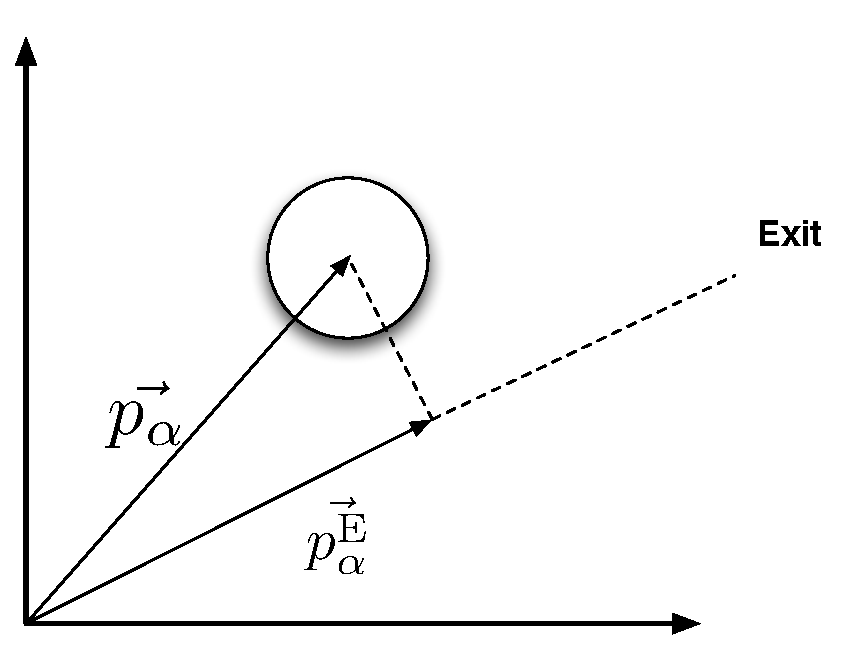
\includegraphics[width=0.5\textwidth]{Figures/NotationOfPedestrian2.pdf}} 
    \caption[Our interpretation of the average velocity]{Our interpretation of 
    the average velocity. The vector pointing from the pedestrian's initial 
    position, $p^i_\alpha$, is projected onto the vector pointing from 
    $p^i_\alpha$ to the pedestrian's target. The length of this projection is 
    divided by the time to yield the average speed.}
    \label{impatience}
\end{figure}

$\langle V_{\alpha}\rangle$ is undefined at $t=0$ as that would result in a 
division by zero. This means that $V^d_\alpha(0)$ is undefined. We correct 
this by defining $V^d_\alpha(0)=V^{Id}_\alpha$. This means that $V^d_\alpha(t)$ 
is defined as follows:

\begin{equation}\label{eqn:cond-define}
    V_{\alpha}^{d} (t) = \left\{ 
    \begin{array}{l l}
        V_\alpha^{Id} & \text{if $t=0$}\\
        \left[ 1 - \eta_{\alpha}(t) \right] 
        V^{Id}_{\alpha} +
        \eta_{\alpha}(t) V_{\alpha}^{\text{max}}
        & \text{if $t > 0$}\\
    \end{array} \right.
\end{equation}

Analysing equations~\eqref{eqn:desired-speed} and \eqref{eqn:impatience}, it 
is clear that as the average speed approaches $V^{Id}_\alpha$ so does the 
desired speed, since $\eta_\alpha(t)\rightarrow0$ for $\langle V_\alpha(t) 
\rangle \rightarrow V^{Id}_\alpha$ which makes $V^d_\alpha(t)$ be dominated by 
$V^{Id}_\alpha$.  


If $\eta_\alpha(t)$ is considered as a function of the average velocity 
instead of the time, it is monotonously decreasing. This means that 
$V^d_\alpha(t)$ considered as a function of the average velocity is 
monotonously decreasing if $V^{\text{max}}_\alpha > V^{Id}_\alpha$, 
monotonously increasing if $V^{\text{max}}_\alpha < V^{Id}_\alpha$, and 
constant if $V^{\text{max}}_\alpha = V^{Id}_\alpha$. This function also has 
the property that $V^d_\alpha(t)=V^{Id}_\alpha$ when $\langle V_\alpha(t) 
\rangle = V^{Id}_\alpha$.

Since $V^{\text{max}}_\alpha$ is set to be larger than $V^{Id}_\alpha$, this 
means that as the average speed goes up, the desired speed goes down.  When 
the desired speed is lower than the actual speed, this will result in a 
negative desired force due to~\eqref{eqn:desired-force}, and vice versa. The 
end result is that the desired force will act as a stabilising force, that 
accelerates the pedestrian when it's moving slower than its desired speed, and 
decelerate it when it's moving faster, but allowing for movement of up to the 
maximum desired speed to ``make up'' for lost time if the pedestrian has been 
slowed down by the other forces acting on it.

The components of the desired force are summarised in 
table~\ref{tbl:desired-force}.

\begin{table}[h]
    \centering
    \begin{tabular}{l l}
        \toprule
        \multicolumn{2}{c}{\textsf{Parameters of the desired force}}\\
        $\overrightarrow{V_{\alpha}}(t)$ & Velocity of pedestrian $\alpha$ 
        at time $t$\\
        $V_{\alpha}^{d}(t)$ & Desired speed of pedestrian $\alpha$ at time 
        $t$\\
        $V_{\alpha}^{Id}$ & Initial desired speed of pedestrian $\alpha$ \\
        $\langle V_{\alpha}(t) \rangle$ & Average speed of pedestrian 
        $\alpha$ \\
        $\tau$& Relaxation time \\
        \bottomrule
    \end{tabular}
    \caption{Summary of parameters of the desired force}
    \label{tbl:desired-force}
\end{table}

\subsection{Repulsion from other pedestrians}\label{seq:repulsion-pedestrians}
The third term on the right hand side of equation \eqref{model} is a summation of all the 
force between pedestrian $\alpha$ and pedestrian $\beta$. The equation we use is taken from a newer article \cite{ABconstant}. We did this because the original article contains two constants that is not given in the articel and in a mail we were adviced, by the authors, to use the values and equation from the new article. 

The function for the repulsion between pedestrians depends on the position vector and the velocity of 
both pedestrians, and it is given by:

\begin{equation}
        \overrightarrow{f_{\alpha \beta }}\left( t \right) = w\left(\phi_{\alpha \beta}\right)\overrightarrow{g}\left(d_{\alpha \beta}(t)\right)
    \label{eq:pedestrianinteraction}
\end{equation}

The two functions that gives the repulsion between the pedestrians is respectively the angel dependece, $ w\left(\phi_{\alpha \beta}\right)$, and the pure force without any angle dependence, $\overrightarrow{g}\left(d_{\alpha \beta}(t)\right)$.

$ w\left(\phi_{\alpha \beta}\right)$ is given as: 

\begin{equation}
    w\left(\phi_{\alpha \beta}\right)=
    \left(
        \lambda_{\alpha} + \left(
            1 - \lambda_{\alpha}
        \right)
		\frac{1+\cos{\phi}}{2}
    \right) 
    \label{angleAB}
\end{equation}

the angle $\phi_{\alpha \beta}$ is the angle between the 
vector pointing from pedestrian $\beta$ to $\alpha$ and the direction in which 
pedestrian $\alpha$ is moving. Cosine to the angle is 

\begin{equation}
\cos \left( \phi \left( t \right) \right)
		= 
	- \overrightarrow{\eta_{\alpha \beta}}
		\left( t \right) 
	\cdot 
\overrightarrow{e_{\alpha}}\left( t \right)
\end{equation}

$\lambda_{\alpha}$ is governing a persons tendency to focus on things happening in front of him 
rather than behind him. It will have a value  $0\leq \lambda_{\alpha}\leq 1$

A value of $\lambda_{\alpha}=1$ means that the force won't depend on the angle. Thus $\alpha$ will react the same to $\beta$ no matter if $\beta$ is in the front or comes from the side or back. A value of $0$ will on the other hand give the maximum angle dependence. We find that $0\leq w\left(\phi_{\alpha \beta}\right)\leq1$ when $-1 \leq \cos \left( \phi \right) \left( t \right) \leq 1$. From this we see that $\alpha$ wont be affected at all if $\beta$ is coming from behind and the force will be maximum when $\beta$ comes directly in the front. It should be noted that in general one will find that the maximum of $w\left(\phi_{\alpha \beta}\right)$ always will be $1$ and the minimum will be equal to $\lambda_{\alpha}$. In very high density calculations $\lambda_{\alpha}$ is often put to $1$, removing $w(\phi_{\alpha \beta})$ and speeding up the simulations.   

% we should make a drawing of this.

The force, without the effect of $w\left(\phi_{\alpha \beta}\right)$, is given as the second term, in the right hand side of equation \ref{eq:pedestrianinteraction}. The function is:  

\begin{equation}
	\overrightarrow{g} 
	\left(
	d_{\alpha \beta}
	\right)
	=
	 A_{\alpha} e^{ \left(\frac{ R_{\alpha \beta} - d_{\alpha \beta}}{B_{\alpha}}\right)}
	\overrightarrow{n}_{\alpha \beta}
	        \label{re}	
\end{equation}

Here $A_{\alpha}$ and $B_{\alpha}$ are constants that can differ for each pedestrian. 
$R_{\alpha \beta}$ is the sum of the radii of $\alpha$ and $\beta$ that is 
$R_{\alpha \beta} = R_{\alpha} + R_{\beta}$. $d_{\alpha \beta}$ is the 
distance from the center of pedestrian $\alpha$ and the center of 
pedestrian $\beta$ and is therefore given by $d_{\alpha \beta} = 
\|\overrightarrow{p_{\alpha}}\left( t \right) - \overrightarrow{p_{\beta}}\left( t \right) \|$.
$\eta_{\alpha \beta}$ is the unit vector pointing from $\alpha$ to $\beta$ 
and it is given by:

\begin{equation}
    \eta_{\alpha \beta} =
        \frac{\overrightarrow{p_{\alpha}}(t) - \overrightarrow{p_{\beta}}(t)}
             {\|\overrightarrow{p_{\alpha}}(t) - \overrightarrow{p_{\beta}}(t) \|}
\end{equation}

\begin{figure}[ht]
    \centering
    {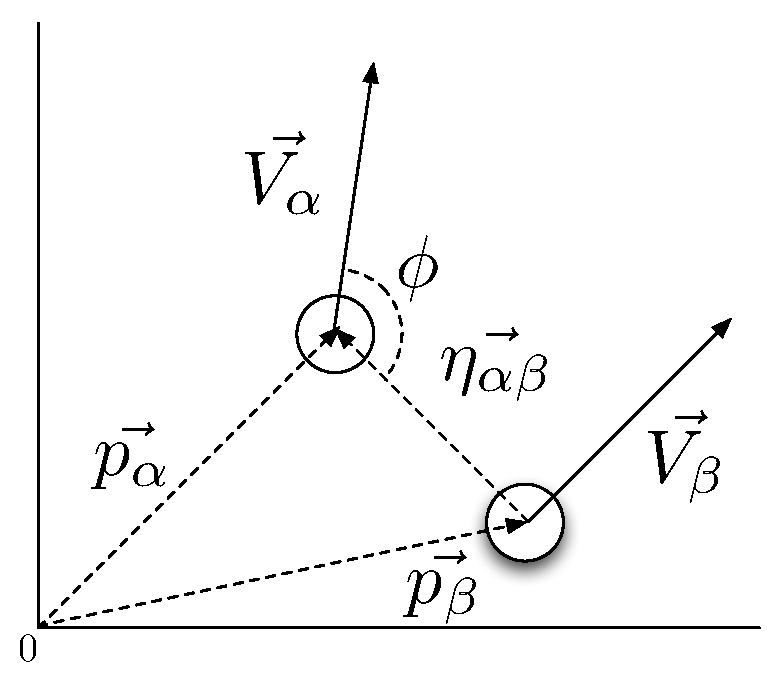
\includegraphics[scale=0.35]{Figures/NotationOfInteraction.pdf}} 
    \caption[Notation of the interaction between two pedestrians]{Illustration of the notation for the interaction between pedestrians.
	     An addition and difference to \ref{NotationOfWall} is that the wall has been replaced by pedestrian $\beta$.
	     $\eta_{\alpha \beta}$ is the vector pointing from $\alpha$ to $\beta$, and $\phi$ is the angle between $\alpha$'s 
	     velocity vector and the vector to $\beta$.}
    \label{fig:NotationOfInteraction}
\end{figure}


%Equation \ref{pedestrianinteraction} is given by two terms. 
%The first term determines how much the the angle between the pedestrians is and how much this angle should affect the force. 
%The constant $\lambda$ is the one controling the importance of the angle.
%The second term reflects the pedestrians tendency to stay at a certain distance 
%from other pedestrians. The constants $A_{\alpha}$, $B_{\alpha}$ is the strength 
%and range of the interaction respectively and controls how big the force will be at a certain distance.  

Taking the norms of both sides of Equation (\ref{re}), we can draw the relation between the value of $\overrightarrow{f_{\alpha\beta}}(t)$ and $ d_{\alpha\beta} $, as shown in Figure 
(\ref{fig:physicalinteraction2}).\\

\begin{figure}[hb]
    \centering
    {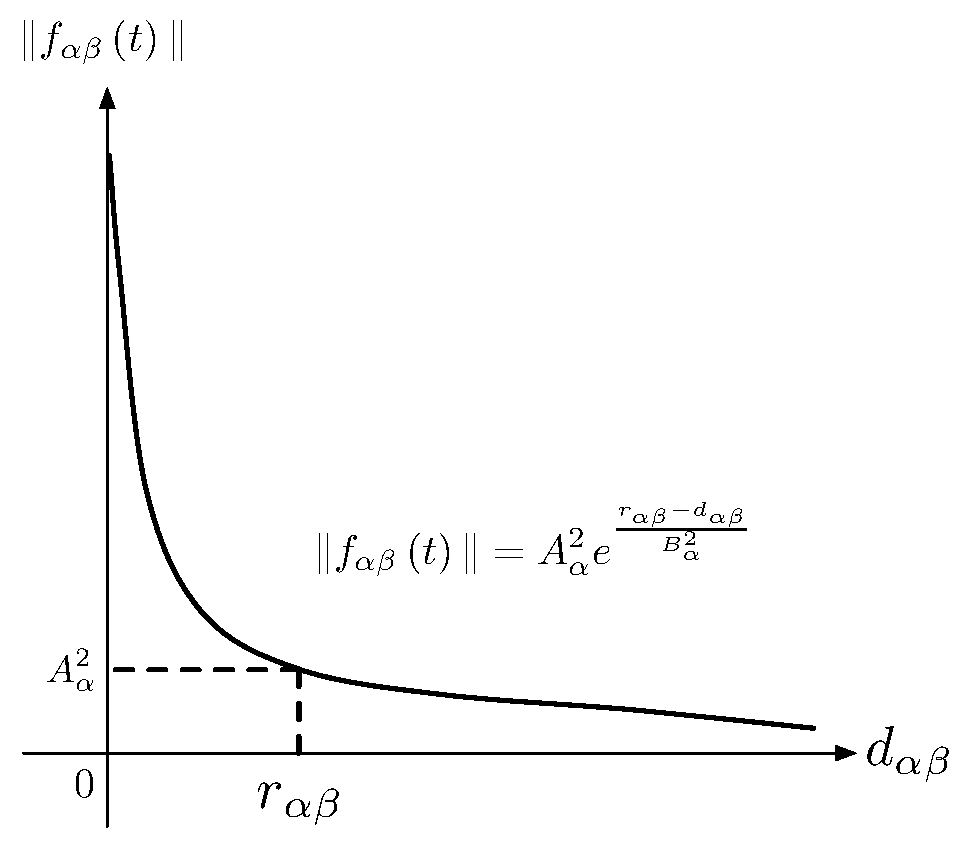
\includegraphics[scale=0.45]{Figures/physicalinteraction.pdf}} 
    \caption[Psysical interaction]{Illustration of the function about the interaction force 
        $f_{\alpha\beta}(t)$ and the distance between two pedestrians
        $d_{\alpha \beta}$. It follows that the smaller the distance between two pedestrians, the greater the interaction force is. }
    \label{fig:physicalinteraction2}
\end{figure}

There is one intersection of the graph and the  axis at:

\begin{equation}
	\left( d_{\alpha \beta} , \| \overrightarrow{f_{\alpha \beta}} \left( t \right) \| \right)
 =
	\left( 0 , A_{\alpha} exp\left( \frac{R_{\alpha\beta} }{B_{\alpha}}\right)  \right) 
\end{equation}

If we put in values for the constants, we will be able to get a maximum value of $ f_{\alpha\beta}(t) $, 
since the distance between pedestrians cannot be negative. Here we take values from \cite{ABconstant} $ A_{\alpha} = 0.42 m/s^{2} $, 
$ R_{\alpha\beta} = 0.6 m $, and $ B_{\alpha} = 1.65 m $, so 
$ f_{\alpha\beta}(t)^{max} < 0.64 m/s^{2} $. It can never be exactly $0.64m/s^2$ since the vector between $\alpha$ and $\beta$ will be undefined when two pedestrians are in the exact same spot.

%TODO: remember to finish this section
%TODO: again lets  have a little summation here. What kinds of dynamics does the
% social interaction part of the model yield.

\begin{center}
\begin{tabular}{lll}
\hline
$d_{\alpha \beta}$& The distance from pedestrian $\alpha$ to $\beta$ &\\
\hline
$R_{\alpha\beta}$& The sum of the radii of pedestrian $\alpha$ and $\beta$ \\
\hline
$\lambda_{\alpha}$& Anisotropy parameter &\\
\hline
$\eta_{\alpha \beta}$& Normal vector pointing from $\beta$ to $\alpha$ \\
\hline
$A_{\alpha}$& Parameter controlling the interaction streanght \\
\hline
$B_{\alpha}$& Parameter controlling the range of the repulsive interaction  \\
\hline
\end{tabular}
\end{center}

\subsection{Repulsion from the walls}\label{seq:repulsion-walls}
The second term on the right hand side of equation \eqref{model} is a force which 
arise from interactions with the walls or other obstacles. It is given by:

\begin{equation}\label{wallpotential}
    \overrightarrow{f_{\alpha B}} \left( \overrightarrow{p_{\alpha}} \right) =
    - \nabla_{\overrightarrow{p_{\alpha}}} U_{B}
    \left( \| \overrightarrow{p_{\alpha}} - \overrightarrow{p_{B}^{\alpha}} \| \right)
\end{equation}

$U_B$ is a repulsive potential and $\|\overrightarrow{p_{\alpha}} - \overrightarrow{p_{B}^{\alpha}}\|$ 
is the distance from the position of pedestrian $\alpha$ to the nearest point on the 
wall as shown in figure \ref{NotationOfWall}. Since $U_B$ is a function of the distance 
$\| \overrightarrow{p_{\alpha}} - \overrightarrow{p_{B}^{\alpha}} \|$, the gradient of $U_B$ tells us in 
which direction this repulsion change the most. It is obvious that the change is 
largest if the pedestrian takes a step directly towards or away from the point in the wall, 
which means that the pedestrian will be pushed directly away from the point in the wall.

\begin{figure}[ht]
\centering
{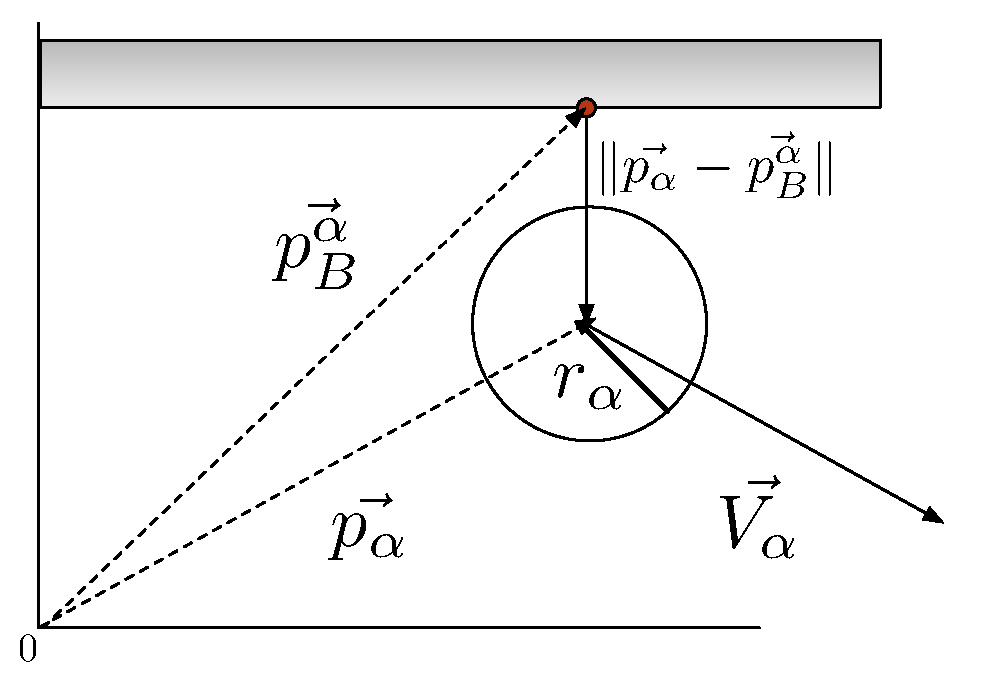
\includegraphics[scale=0.35]{Figures/NotationOfWall.pdf}} 
\caption[Notation of the interaction between an pedestrian and a wall]{The illustration shows the mathematical notation for the interaction with walls used. The circle is pedestrian $\alpha$ with radius $R_{\alpha}$, $\overrightarrow{p_{\alpha}}$ is the position vector for $\alpha$, the grey box on the top is the wall, $\overrightarrow{p_{B}^{\alpha}}$ is the position vector for the closest part of the wall to $\alpha$, $\left( \| \overrightarrow{p_{\alpha}} - \overrightarrow{p_{B}^{\alpha}} \| \right)$ is the smallest distance from $\alpha$ to the wall and $\overrightarrow{V_{\alpha}}$ is the velocity vector for $\alpha$.}
\label{NotationOfWall}
\end{figure}

In order to do the actual calculation we need to know the explicit expression for 
$ \| \overrightarrow{p_{\alpha}} - \overrightarrow{p_{B}^{\alpha}} \|$. First we need to find point on the wall 
that is perpendicular to $\alpha$ as this will be the nearest point to $\alpha$. If we define 
the wall as a vector, $\overrightarrow{W}$ going from a point in space $w_1$ to another point $w_2$, then 
we can find the projection of $\alpha$'s position onto the wall and this projection will be 
$\overrightarrow{p_{B}^{\alpha}}$. This projection is given by:

\begin{equation}\label{wall}
\overrightarrow{p_{B}^{\alpha}}=\frac{\overrightarrow{p_{\alpha}}\cdot \overrightarrow{W}}{\| \overrightarrow{W} \|^2}\overrightarrow{W}
\end{equation}

With this we now have the two points we need to calculate $\|\overrightarrow{p_{\alpha}} - \overrightarrow{p_{B}^{\alpha}}\|$ 
since the position of $\alpha$ is know at all times.

With the explicit expression for $ \| \overrightarrow{p_{\alpha}} - \overrightarrow{p_{B}^{\alpha}} \| $ 
in hand we are able to calculate $\overrightarrow{f_{\alpha B}} \left( \overrightarrow{p_{\alpha}} \right)$ from 
Equation \ref{wallpotential}, as long as the expression for the potential function 
$U_{B}\left( \| \overrightarrow{p_{\alpha}} - \overrightarrow{p_{B}^{\alpha}} \| \right)$ is given. This is 
however not the case in the main article we are working with. In another articles \cite{ABconstant} by 
the same author the repulsive potential from the wall is given by: 

\begin{equation}
U_{B} \left( \| \overrightarrow{p_{\alpha}} - \overrightarrow{p_{B}^{\alpha}} \| \right) =
U^0_{\alpha B} e^{- \| \overrightarrow{p_{\alpha}} - \overrightarrow{p_{B}^{\alpha}} \| / R_{\alpha} }
\end{equation}

where $U^0_{\alpha B}$ is a constant and $R_{\alpha}$ is the radius of a pedestrian $\alpha$.
In that case, the repulsive force on pedestrian $ \alpha $ from the wall is:

\begin{equation}
    \overrightarrow{f_{\alpha B}} \left( \overrightarrow{p_{\alpha}} \right) =
    - \nabla_{\overrightarrow{p_{\alpha}}} U_{B}
    \left( \| \overrightarrow{p_{\alpha}} - \overrightarrow{p_{B}^{\alpha}} \| \right)\\
=-\left( \frac{\partial}{\partial x_{\alpha}}U_{B}( \| \overrightarrow{p_{\alpha}} - \overrightarrow{p_{B}^{\alpha}} \|), \frac{\partial}{\partial y_{\alpha}}U_{B}( \| \overrightarrow{p_{\alpha}} - \overrightarrow{p_{B}^{\alpha}} \|)\right)
\end{equation}

Calculating the derivatives we assume that we now the direction of the force, so the differentiation will be one dimensional

\begin{equation}
\begin{split}
f_{\alpha B} \left( \overrightarrow{p_{\alpha}} \right) 
 = -\frac{\partial}{\partial \| \overrightarrow{p_{\alpha}} - \overrightarrow{p_{B}^{\alpha}} \|}U^0_{\alpha B} e^{- \| \overrightarrow{p_{\alpha}} - \overrightarrow{p_{B}^{\alpha}} \| / R_{\alpha} }
\end{split}
\end{equation}

The differentiation then gives: 

\begin{equation}
    f_{\alpha B} \left( \overrightarrow{p_{\alpha}} \right) 
=\frac{1}{R_{\alpha}} U^0_{\alpha B} e^{- \| \overrightarrow{p_{\alpha}} - \overrightarrow{p_{B}^{\alpha}} \| / R_{\alpha} }
\end{equation}

To get the direction of the force, we multiply it with the unit vector of the vector from the wall to $\alpha$ since the force will have the same direction 
\begin{equation}\label{eqn:wall-repulsion}
\overrightarrow{f_{\alpha B}}=\frac{1}{R_{\alpha}} U^0_{\alpha B} e^{- \| \overrightarrow{p_{\alpha}} - \overrightarrow{p_{B}^{\alpha}} \| / R_{\alpha} }\frac{\left(p_{\alpha x}-p_{Bx}^{\alpha },p_{\alpha y}-p_{By}^{\alpha }\right)}{ \| \overrightarrow{p_{\alpha}} - \overrightarrow{p_{B}^{\alpha}} \| }
\end{equation}

The exponential function will always lay between 0 and  1:

\begin{equation}
0 < e^{ -\| \overrightarrow{p_{\alpha}} - \overrightarrow{p_{B}^{\alpha}} \| /R_\alpha} < 1
\end{equation}

Which leads to:

\begin{equation}
0< U_{B} \left( \| \overrightarrow{p_{\alpha}} - \overrightarrow{p_{B}^{\alpha}} \| \right) < U^0_{\alpha B}
\end{equation}

We can see that this force act in the following way: $\overrightarrow{f_{\alpha B}}$ tends to 0 as the distance 
$\| \overrightarrow{p_{\alpha}} - \overrightarrow{p_{B}^{\alpha}} \|$ gets large, meaning that a pedestrian in a reasonably 
distance from the wall will feel a diminishing force. $\overrightarrow{f_{\alpha B}}$ tends to $U^0_{\alpha B}$ 
as the distance $ \| \overrightarrow{p_{\alpha}} - \overrightarrow{p_{B}^{\alpha}} \|$ tends to $0$ the pedestrian will be 
pushed, with some force depending on $U^0_{\alpha B}$, away from the wall. The negative of the force 
means that when the potential between wall and pedestrian rises so will the force, but in the opposite 
direction meaning that the pedestrian will be pushed away. This can be understood as if the pedestrian 
is trying to avoid the wall as it is expected from real life situations. \cite{social-force}. %real references, please.

\begin{center}
\begin{tabular}{lll}
\hline
$\overrightarrow{p_{\alpha}^{\text{B}}}$& Vector pointing from origo to the point on the wall nearest to pedestrian alpha &\\
\hline
$\overrightarrow{W}$& Vector representing the wall &\\
\hline
$U_{B}$ & Repulsive potential from the wall\\
\hline
$U^{0}_{\alpha B}$ & Constant representing pedestrian alpha's tendency to avoid walls\\
\hline
$R_{\alpha}$& Repulsive potential from the wall\\
\hline
\end{tabular}
\end{center}

\subsection{Summary of the model}
\begin{figure}[hb] %with some more comments i think that this figure could serve as a summation of the entire section
    \centering
    {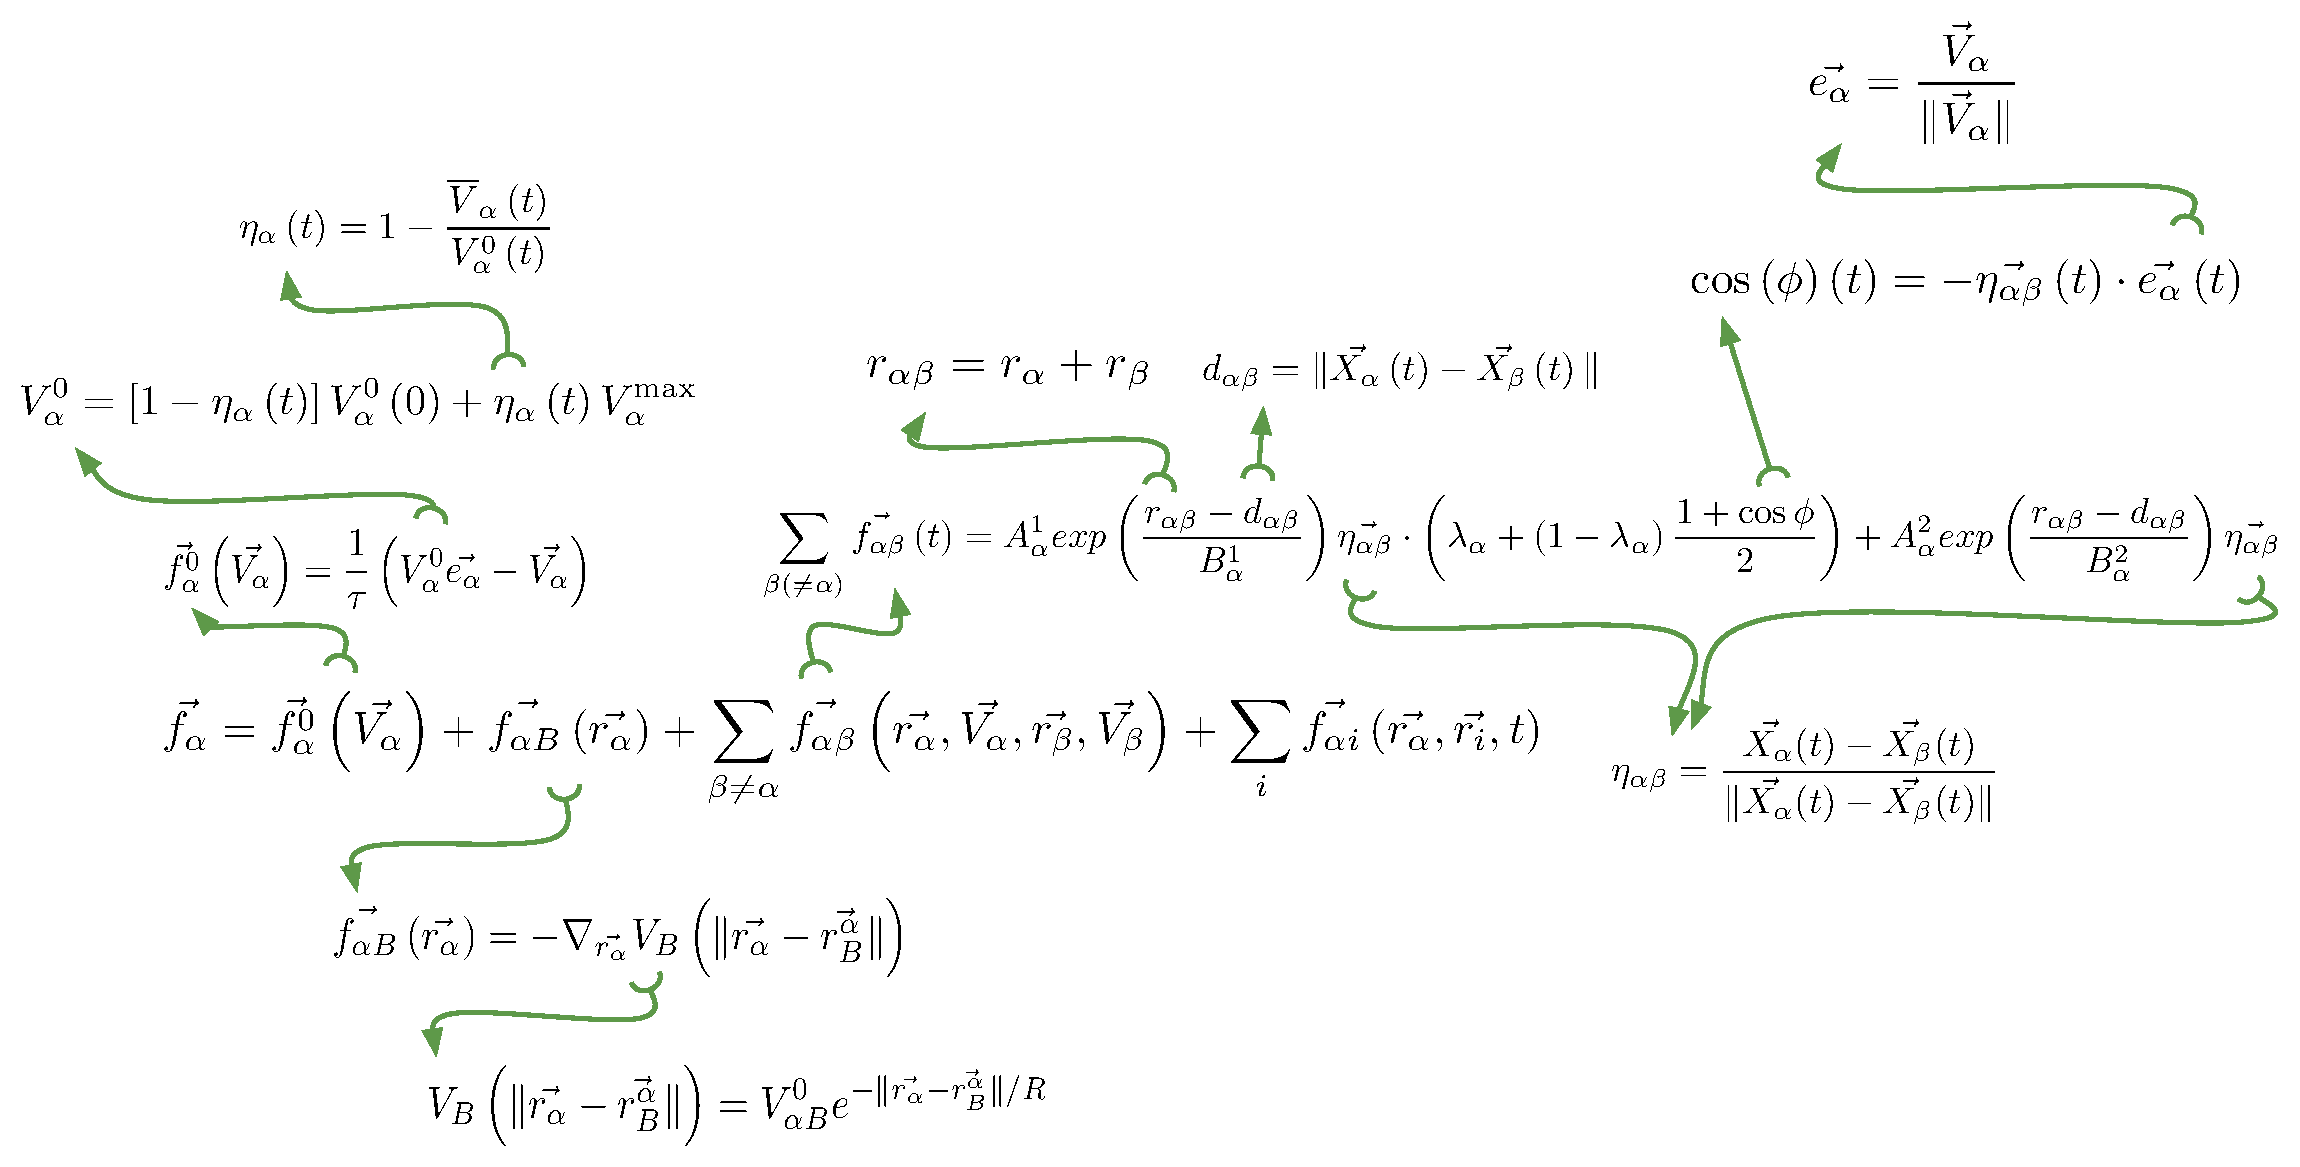
\includegraphics[scale=0.35]{Figures/overview.pdf}} 
    \caption[Overview of the model]{Illustration of an overview of how the model is put together. The different equations and their notation is written to give the 
	     reader an overview of how the model looks like.}
    \label{overview}
\end{figure}

\begin{center}
\begin{tabular}{lll}
\hline
$\overrightarrow{f_{\alpha}^{0}}$ & the desired force &\\
\hline
$\overrightarrow{f_{\alpha B}}$ & the repulsive force from walls &\\
\hline
$\overrightarrow{f_{\alpha \beta}}$ & the repulsion from other pedestrians\\
\hline
$\overrightarrow{f_{\alpha i}}$& the attractive force\\
\hline
$\overrightarrow{V_{\alpha}}$ & The actual velocity of pedestrian alpha &\\
\hline
$V_{\alpha}^{0}(t)$ & The desired speed of pedestrian alpha &\\
\hline
$V_{\alpha}^{0}(0)$ & The initial desired speed of pedestrian alpha &\\
\hline
$\overline{V_{\alpha}(t)}$ & The average speed of pedestrian alpha &\\
\hline
$\overrightarrow{p_{\alpha}}$ & The position vector of pedestrian alpha\\
\hline
$e_{\alpha}$& The desired direction of pedestrian alpha\\
\hline
$\tau$& The relaxation time &\\
\hline
$\overrightarrow{p_{\alpha}^{\text{B}}}$& Vector pointing from origo to the point on the wall nearest to pedestrian alpha &\\
\hline
$\overrightarrow{W}$& Vector representing the wall &\\
\hline
$U_{B}$ & Repulsive potential from the wall\\
\hline
$U^{0}_{\alpha B}$ & Constant representing pedestrian alpha's tendency to avoid walls\\
\hline
$R_{\alpha}$& Repulsive potential from the wall\\
\hline
$d_{\alpha \beta}$& The distance from pedestrian $\alpha$ to $\beta$ &\\
\hline
$R_{\alpha\beta}$& The sum of the radii of pedestrian $\alpha$ and $\beta$ \\
\hline
$\lambda_{\alpha}$& Anisotropy parameter &\\
\hline
$\eta_{\alpha \beta}$& Normal vector pointing from $\beta$ to $\alpha$ \\
\hline
$A_{\alpha}$& Parameter controlling the interaction streanght \\
\hline
$B_{\alpha}$& Parameter controlling the range of the repulsive interaction  \\
\hline
$d_{\alpha \beta}$& The distance from pedestrian $\alpha$ to $\beta$ &\\
\hline
$R_{\alpha\beta}$& The sum of the radii of pedestrian $\alpha$ and $\beta$ \\
\hline
$\lambda_{\alpha}$& Anisotropy parameter &\\
\hline
$\eta_{\alpha \beta}$& Normal vector pointing from $\beta$ to $\alpha$ \\
\hline
$A_{\alpha}$& Parameter controlling the interaction streanght \\
\hline
$B_{\alpha}$& Parameter controlling the range of the repulsive interaction  \\
\hline
\end{tabular}
\end{center}

We have now seen the explicit mathematical expression for the social forces 
as well as explained how this affects the behavior of the pedestrians. To get an 
overview of how the model is put together look a figure \ref{overview} with 
the aid of table. In section \ref{sec:assessment} 
we discuss some of the models features in more detail as well as some features 
that the model does not have. For the implementation of the model see section \ref{sec:simulation}.
